\chapter{Arbejdsproces}\label{Arbejdsproces}
Gruppens måde at arbejde på igennem forløbet har varieret, der er både blevet arbejdet individuelt, hjemmearbejde og arbejde på tværs af gruppen. Til sidst i dette kapitel vil der blive reflekteret over hvordan arbejdsprocessen har fungeret.


\section{Arbejdspapir}\label{Arbejdspapir}
Arbejdspapir blev lagt op på GoogleDrev hver gang nogen havde lavet noget. Det gjorde det muligt for alle gruppemedlemmer at se hvad hvert enkelt medlem havde lavet, men også give dem mulighed for at læse det de andre havde skrevet.

\section{Programmering}\label{Programmering}

Da gruppen nåede til at programmere programmet, var det meningen at gruppen skulle dele sig op i mindre delgrupper, for at lave forskellige dele af programmet. Dog endte det med at gruppen programmerede på tværs i programmet, men samtidig var der nogle medlemmer som arbejdede sammen om forskellige dele. Flere dele af programmet blev også skrevet af enkelte medlemmer, eftersom det var et omfang som enkelte personer kunne udføre. I starten af projektet blev det besluttet at lave et code-review hver mandag, når programmeringsfasen var igang. Dog blev dette ikke helt tilfældet, det endte med at gruppen lavede et code-review, når gruppen følte der var brug for det i stedet. 


\section{Metode}\label{Metode}

Dette afsnit har til formål at give et indblik i hvordan der er blevet arbejdet metodisk og videnskabeligt igennem projektet fra det initierende problem, og igennem rapporten til der opnås en endelige konklusionen. Metode kapitlet har til formål at gøre det muligt for læseren at få indsigt, hvordan vi igennem hele forløbet har arbejdet os frem til et færdigt produkt, og hvordan der overordnet er blevet arbejdet for at nå frem til dette produkt. 

\subsection{Brainstorm}
Med udgangspunkt i hovede-emnet simuleringer var første proces, at undersøge mulige kategorier af under-emner, hvor man kunne se simulering som værende en del af en løsning til at afvikle et problem, samt et under-emne som et flertal synes kunne være interessant at arbejde med. Først blev gruppens medlemmer bedt at undersøge hvorvidt om det var muligt at finde noget brugbart materiale omkring de emner som de havde forslået og havde i tankerne. Hvorefter gruppens medlemmer fremlagde det som de havde fundet frem til, så det var muligt at vælge ved afstemning hvilket emne et flertal kunnes samles omkring til at indskrænke os. 

\begin{figure}[h]
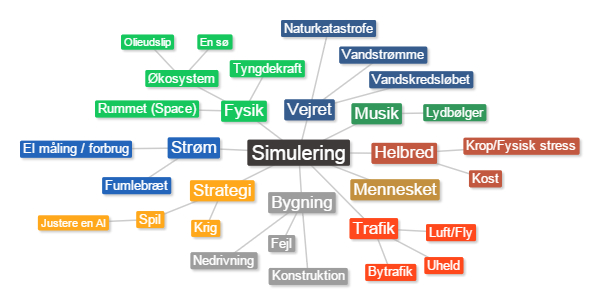
\includegraphics[scale=0.35]{Simulering-Brainstorm}
\centering
\caption{Gruppens brainstorm af simulering}\label{Simulering_Brainstorm}
\end{figure}

\subsection{Kildekritik}
For at finde frem til relevant information, er der blevet taget udgangspunkt i kilder med ophav fra statslige instanser eller anerkendte virksomheder og organisationer, for at sikre informationernes gyldighed og troværdighed. Dette vil det også være muligt at kunne kontakte kilderne for uddybende spørgsmål, skull
e der opstå tvivl om dele af informationen eller indsamlet data i det anvendte information. Ydermere er der blevet forsøgt at finde den nyeste tilgængelige information, for at sikre at den indsamlede data stadigvæk er brugbart og gyldigt. Fordi flere af de anvendte kilder kunne have en tendens, er den præsenteret information blevet kritisk overvejet efter hvorvidt det forholder sig objektivt eller om det er blevet fremstillet til at opnå noget for egen vinding eller et specielt mål.

\section{Reflektion over arbejdsprocessen}\label{Reflektion-over-arbejdsprocessen}
Arbejds processen var generelt langsom i starten af projektet, da gruppen ikke selv helt vidste hvor de ville hen med forløbet. Dette skyldes at i starten af projektet arbejdede gruppen altid i grupperum fra 8.15 til 16.00. Gruppen fandt ud af, at ikke alle gruppemedlemmer havde lyst til dette, samtidig mistede gruppen koncentrationen, når vi var i grupperummet. Dette skyldes at flere medlemmer altid sad og lavede noget andet, så som at snakke om diverse serier eller andet ikke gruppe relateret. Gruppen kom på en løsning, som var at arbejde hjemme, på denne måde ville gruppemedlemmer ikke blive forstyret af andre, dette gjorde også at der blev arbejdet på projektet. Gruppen uddelte opgaver ud til individueller medlemmer, når disse opgaver var lavet så ville gruppen gennemgå det sammen. Dette fungerede godt, fordi hele gruppen var med ind over hele rapporten. 

\vspace{5mm}

I programmerings fasen var flere gruppemedlemmer bagud i starten, dette skyldes at enkelte medlemmer havde programmeret på programmet i starten. På denne måde var flere medlemmer bagud, da de ikke kendte til det kode der allerede var blevet skrevet. I fremtiden vil gruppen derfor sørger for at alle gruppemedlemmer er med på programmeringsdelen fra start af. Dette vil gøres ved at alle gruppemedlemmer planlægger programmets struktur sammen, inden programmeringsfasen begynder. Samtidig skal gruppen dele sig op i 2 eller 3 mands grupper, og disse grupper skal blande sig hver uge. På denne måde vil alle gruppemedlemmer have en chance for at være med over hele programmet.  